\documentclass{article}%
\usepackage[T1]{fontenc}%
\usepackage[utf8]{inputenc}%
\usepackage{lmodern}%
\usepackage{textcomp}%
\usepackage{lastpage}%
\usepackage{authblk}%
\usepackage{graphicx}%
%
\title{Ubiquitin{-}conjugating enzyme complex Uev1A{-}Ubc13 promotes breast cancer metastasis through nuclear factor{-}\_B mediated matrix metalloproteinase{-}1 gene regulation}%
\author{Jennifer Smith}%
\affil{Osteoncology Center, IRCCS Istituto Scientifico Romagnolo per lo Studio e la Cura dei Tumori (I.R.S.T.), I{-}47014 Meldola (FC), Italy, Biosciences Laboratory, IRCCS Istituto Scientifico Romagnolo per lo Studio e la Cura dei Tumori (I.R.S.T.), I{-}47014 Meldola (FC), Italy}%
\date{01{-}01{-}2009}%
%
\begin{document}%
\normalsize%
\maketitle%
\section{Abstract}%
\label{sec:Abstract}%
The lungs are the lungs! U.S. Centers for Disease Control and Prevention offers many excellent resources to provide information about respiratory diseases, including pulmonary disease and risk factors for lung disease in the United States, with follow{-}up information on how these diseases impact the health of the lung and the community, including reduced lung function, increased severity, a reduction in lung capacity, decreased length of life, premature death, increased risk of heart disease, high cholesterol and stroke, smoking{-}related lung diseases and cardiovascular disease. In addition, we frequently publish important clinical trials data in infectious diseases in order to improve lung function and provide important health and medical information about secondary and tertiary pulmonary diseases.\newline%
For more information, visit www.lung.gov or www.link.net/lung.html\newline%
The Centers for Disease Control and Prevention (CDC) encourages providers and individuals to follow Food and Drug Administration (FDA) guideline of at least 80 mg/day of sodium when planning as sodium intake.\newline%
For further information on sodium/alcohol intake, visit www.metabolism.gov/inhalation/meso{-}sals.html or www.link.net/ohm .\newline%
The Centers for Disease Control and Prevention(CDC) serves one of the worlds largest public health health care systems. In 2009, our government, agencies, partner organizations and private sector entities shared more than 67 million infections, 65,000 deaths, 3,400 hospitalizations and 17 million children ill with more than 250,000 new cases of infectious diseases.\newline%
Join the free Follow{-}Up People Locator here for topics the CDC works with to promote community health. For more information about the CDC web site visit http://www.cdc.gov/health/childhood/index.htm.

%
\subsection{Image Analysis}%
\label{subsec:ImageAnalysis}%


\begin{figure}[h!]%
\centering%
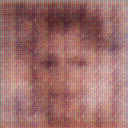
\includegraphics[width=150px]{500_fake_images/samples_5_439.png}%
\caption{A Black And White Photo Of A Black And White Photo}%
\end{figure}

%
\end{document}